\lecture{12}{5. Marts 2025}{Composites, Pt. 1 -- Materials and general rules}

\section{Composites}
The following lectures are going to be focused on composites.
\begin{definition}[Composites]
  A \textit{composite} is a combination of two or more individual materials. The hope of combining materials like this is that the combined properties of the material fit better for the desired use case than either of the individual materials would individually. 
\end{definition}
Composites are used in a wide range of materials. E.g. polymer based carbon finer is used in the fields of:
\begin{itemize}
  \item Acoustics
  \item Textile and Paper industry
  \item Aerospace and Aircraft industry
  \item Portable power sources
  \item Energy production
  \item Sports equipment
  \item Civil engineering
  \item Automotive industry
\end{itemize}

\subsection{The architecture of composites}
A composite can be thought of as an artificially made (as composites do not exist in nature) multiphase material. The phases in a composite are normally split into the two categories:
\begin{itemize}
  \item \textbf{Matrix:} The continuous phase
  \item \textbf{Dispersed:} Is discontinuous and surrounded by the matrix
\end{itemize}
These two different phases that exist in all composites are shown on \textbf{\autoref{fig:f12_1}}.
\begin{figure} [ht]
  \centering
  \caption{The architecture of a composite}
  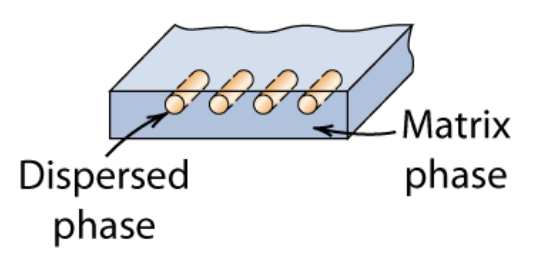
\includegraphics[width=0.25\linewidth]{./figures/f12_1.png}
  \label{fig:f12_1}
\end{figure}

The purpose of the matrix phase is to transfer stress to the dispersed phase and generally protect the dispersed phase from the environment. These mainly come as either metals (MMC), ceramics (CMC) or polymers (PMC). The dispersed phase is normally either made of particles or fibers (although it is sometimes made from structural components such as sandwich panels or nanoparticles as well) and its purpose depends a bit on the type of matrix:
\begin{itemize}
  \item MMC: The purpose of the dispersed phase is often to increase the yield strength $\sigma_y$, increase the creep resistance and to increase the tensile strength.
  \item CMC: The purpose of the dispersed phase is often to boost fracture toughness $K_{Ic}$
  \item PMC: The purpose of the dispersed phase if to enhance stiffness $E$, yield strength $\sigma_y$ and creep resistance.
\end{itemize}

\begin{figure} [ht]
  \centering
  \caption{Classification of composites with the part mentioned in this lecture encased in a blue rectangle.}
  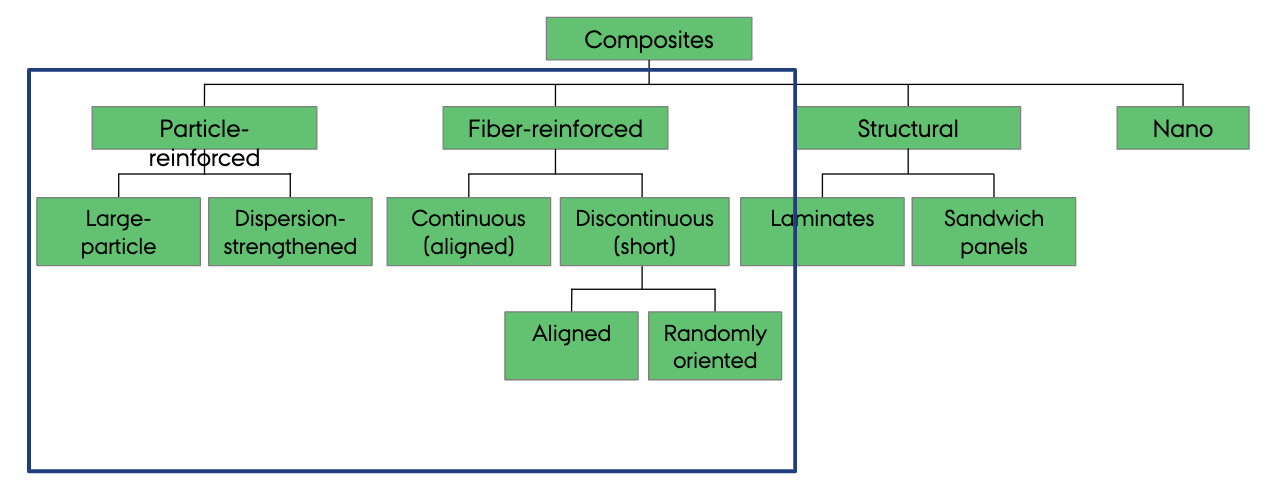
\includegraphics[width=0.75\linewidth]{./figures/f12_2.png}
  \label{fig:f12_2}
\end{figure}
On \textbf{\autoref{fig:f12_2}} the most common way to classify composites is shown. This lecture will focus on particle- and fiber-reinforced composites (the part encased in the blue rectangle).


\subsection{Particle-reinforced composites}
On \textbf{\autoref{fig:f12_3}} three examples of particle reinforced composites in common usage are shown.
\begin{figure} [ht]
  \centering
  \caption{Examples of particle reinforced composites}
  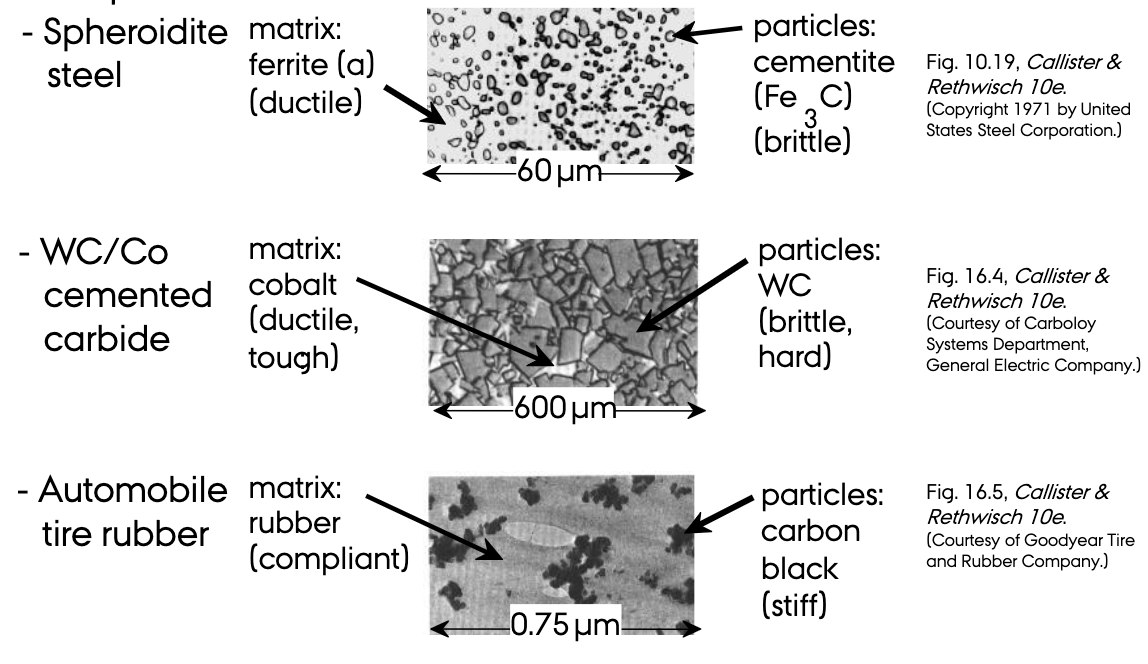
\includegraphics[width=0.6\linewidth]{./figures/f12_3.png}
  \label{fig:f12_3}
\end{figure}
The top picture is of Spheroidite steel. In spheroidite steel the matrix is ferrite (which is relatively ductile) and the dispersed phase is particles of cementite ($\mathrm{Fe}_3 \mathrm{C}$; which is hard and brittle). Here the cementite particles strengthen the steel, while the ferrite matrix provides overall toughness. 

The second picture is of $\mathrm{WC} / \mathrm{Co}$ (Tungsten Carbide in Cobalt). Here the matrix is made of cobalt, which is a ductile and tough metal. The  dispersed phase is particles of tungsten carbide, which is extremely hard and brittle. The Tungsten Carbide provides high hardness and wear resistance, whilst the Cobalt helps the material retain some toughness. This mixture is a part of a larger group of ``cemented carbides'' which are commonly used for cutting tools and other high-wear applications.
The last pircture is of Automobile Tire Rubber. In this case, the matrix is rubber, which is compliant and elastic. The dispersed phase consists of particles of carbon black which is stiff and enhances wear resistance and mechanical strength. 

Common for all the three above exambles is that the \textit{matrix} phase is generally more ductile or compliant, while the \textit{particles} are stiffer or harder. This is true for most composites.

\subsubsection{Elastic modulus of Particle-Reinforced Composites}
To prdict an overall elastic modulus for a composite material $E_c$ two extreme bounds known as \textit{rules of mixture} are commonly used.

\paragraph{Voigt Model (Upper Bound)} The Voigt model assumes that both of the phases in the material experience equal strain (i.e. they elongate the same under load). This is typically thought of as the ``best case'' scenario for stiffness. The predicted stiffness from the Voigt model can be found as
\[ 
E_c = V_m E_m + V_p E_p
.\]

\paragraph{Reuss Model (Lower Bound)} The Reuss model assumes that both of the phases in the composite experience the same stress under a load (also called the \textit{isostress condition}). This represents the ``worst-case'' scenario for stiffness and the predicted stiffness can be calculated as
\[ 
\frac{1}{E_c} = \frac{V_m}{E_m} + \frac{V_p}{E_p}
.\]
\begin{figure} [ht]
  \centering
  \caption{Determining a predicted elastic modulus of a composite}
  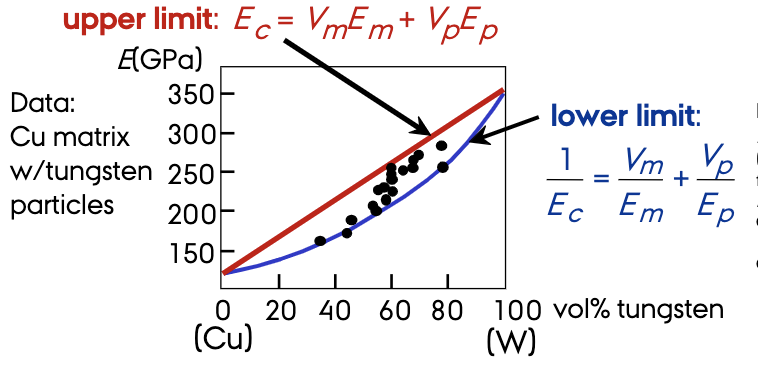
\includegraphics[width=0.5\linewidth]{./figures/f12_4.png}
  \label{fig:f12_4}
\end{figure}
Real composites typically fall between these two bounds as shown on \textbf{\autoref{fig:f12_4}}.


\subsection{Fiber-reinforced composites}
Fibers are very strong in tension and are therefore often used in composites -- This can provide a significant strength-boost to the composite. A few different fiber types are in common use these include (but are not limited to):
\begin{itemize}
  \item \textbf{Whiskers:} Extremely strong single crystals (e.g. silicon carbide, silicon nitride, or graphite). These crystals have high crystal perfection and are therefore extremely strong but also expensive and they can be difficult to disperse.
  \item \textbf{Fibers:} Usually polycrystalline or amorphous (e.g. alumina, aramid, boron, UHMWPE) polymers or ceramics. These are typically used in polymer-matrix composites.
  \item \textbf{Wires:} Metallic wires (e.g. steel, tungsten) can be used where high temperature or electrical conductivity is important.
\end{itemize}

\subsubsection{Fiber alignment}
\begin{figure} [ht]
  \centering
  \caption{Three types of fiber alignment}
  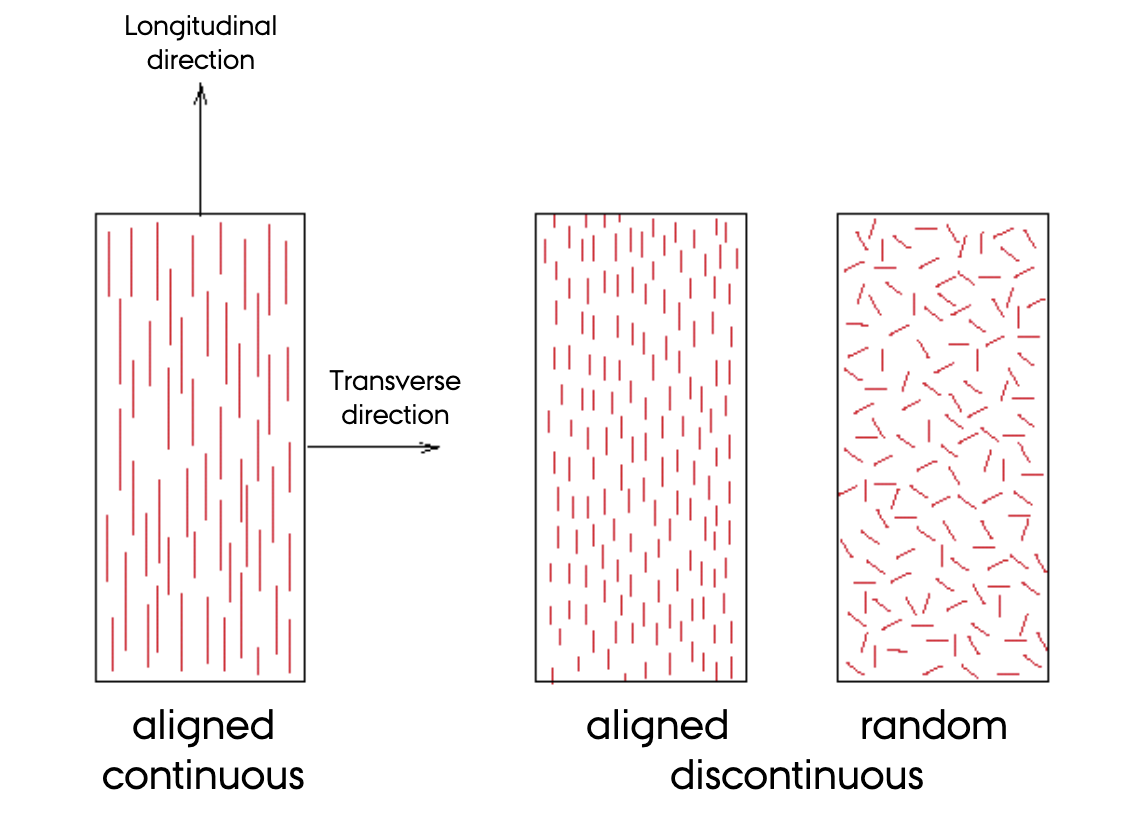
\includegraphics[width=0.5\linewidth]{./figures/f12_5.png}
  \label{fig:f12_5}
\end{figure}
In general three types of fiber alignment are in use. These are shown on \textbf{\autoref{fig:f12_5}}. If you use continuous (long) fibers these are typically aligned within the matrix. This gives great strength and stiffness when the load is parallel to the fibers but very low strength in the direction transverse to the fibers as the fibers do not carry load effectively sideways.

If you instead use discontinuous (short) fibers you can choose to either align these or have them in random directions. When aligned some of the benefits from the continuous fibers are retained. When random the properties of the material are more isotropic (similar in all directions) but the composite does not reach the same peak strength as aligned fibers.

\subsubsection{Critical fiber length}
For effective stiffening and strengthening the fiber length in the composite should surpass the critical fiber length $l_c$ given by
\[ 
l_c = \frac{\sigma_f d}{2 \tau_c}
.\]
Where $\sigma_f$ is the ultimate tensile strength of the fibers, $d$ is the fiber diameter and $\tau_c$ is the shear-strength of the fiber-matrix interface. This is a result of the fact that longer fibers transfor the stress from the matrix much more efficiently than short fibers.

\subsubsection{Estimating the elastic modulus and strength for fiber reinforced composites}
For continuous and aligned fibers it is reasonable to assume that the fibers and the matrix experience the same strain (isostrain; Voigt model). That is
\[ 
\sigma_c = \sigma_m V_m + \sigma_f V_f \quad \text{and} \quad \epsilon_c = \epsilon_m = \epsilon_f
.\]
These van be combined to find the longtitudal modulus for a composite with continuous fibers as
\[ 
E_{cl} = E_m V_m + E_f V_f
.\]

In transverse loading the fibers carry less of the load and in this case we instead assume isostress (Reuss model). That is
\[ 
\epsilon_c = \epsilon_m V_m + \epsilon_f V_f \quad \text{and} \quad \sigma_c = \sigma_m = \sigma_f = \sigma
.\]
These can be combined to give the transverse modulus for a continuous fiber reinforced composite as
\[ 
\frac{1}{E_{ct}} = \frac{V_m}{E_m} + \frac{V_f}{E_f} \implies E_{cf} = \frac{E_m E_f}{V_m E_f + V_f E_m}
.\]

Empirically we have also been able to make estimates of $E_{cd}$ for discontinuous fibers. This is however only valid for fiber lengths $< 15 \frac{\sigma_f d}{\tau_c}$. If this is respected the elastic modulus in the fiber direction is
\[ 
E_{cd} = E_m V_m + k E_f V_f
.\]
Where $k$ is the ``efficiency factor'', which is:
\begin{itemize}
  \item Aligned:
    \begin{itemize}
      \item Aligned parallel $k = 1$
      \item Aligned perpendicular $k = 0$
    \end{itemize}
  \item Random:
    \begin{itemize}
      \item Random 2D $k = \frac{3}{8}$
      \item Random 3D $k = \frac{1}{5}$
    \end{itemize}
\end{itemize}

The estimated strength $\sigma_{cd}^{*}$ for a fiber-reinforced composite with discontinuous fibers is:
\begin{itemize}
  \item When $l > l_c$:
    \[ 
    \sigma_{cd}^{*} = \sigma_f^{*} V_f \left( 1 - \frac{l_c}{2l} \right) + \sigma_m' \left( 1 - V_f \right)
    .\]
  \item When $l < l_c$:
    \[ 
    \sigma_{cd'}^{*} = \frac{l \tau_c}{d} V_f + \sigma_m' \left( 1 - V_f \right)
    .\]
\end{itemize}
